\documentclass[14pt,xcolor=pdftex,dvipsnames,table]{beamer}

% Specify theme
\usetheme{Madrid}
% See deic.uab.es/~iblanes/beamer_gallery/index_by_theme.html for other themes
\usepackage{caption}
\usepackage{tikz}
\usepackage{multirow}
% Specify base color
\usecolortheme[named=OliveGreen]{structure}
% See http://goo.gl/p0Phn for other colors

% Specify other colors and options as required
\setbeamercolor{alerted text}{fg=Maroon}
\setbeamertemplate{items}[square]

% Title and author information
\title{Carry-trade and transition}
\author{Rob Hayward}


\begin{document}

\begin{frame}
\titlepage
\end{frame}

\begin{frame}{Outline}
\tableofcontents
\end{frame}

\section{Introduction}
\begin{frame}{The carry-trade}
Attempts to take advantage of the breakdown in uncovered interest parity
\pause
\begin{block}{}
\begin{equation*}\label{eqref:carry}
y_{t+1} = \frac{(i^* - i)}{\Delta s_{t+1}}
\end{equation*}
\end{block}
Where $y_{t+1}$ are the profits from the carry trade, $i^* - i$ is the interest rate differential (overseas less home) and $\Delta s_{t+1}$ is the change in the exchange rate.    
\end{frame}

\begin{frame}{Failure of UIP}
\begin{block}{}
\begin{equation*}
E[\Delta s_t] = \alpha + \beta (i^* - i) + \varepsilon
\end{equation*}
\end{block}
\pause
Where $E[s_t]$ is the expected change in the exchange rate; $i$ is the domestic interest rate; $i^*$ is the overseas interest rate; $f_s$ is the forward rate. 
\begin{block}{}
\begin{equation*}
\Delta s_t = \alpha + \beta f_s + \varepsilon
\end{equation*}
\end{block}
\end{frame}

\begin{frame}{Risk}
The explanation assumes that there is risk
\pause
\begin{block}{}
\begin{equation*}
\Delta s_t = i^* - i - rp
\end{equation*}
\end{block}
\pause
Where $rp$ is the risks premium
\end{frame}

\begin{frame}{Peso effects}
If $s_t$ is the exchange rate, the peg is state $s^0$ with the probability of a discrete devaluation to $s^1$ of $\pi$, the expected depreciation is
\begin{block}{}
\begin{equation*}
E[s_{t+1}|\Omega_t] = \pi_ts^1 + (1 - \pi_t)s^0
\end{equation*}
\end{block}
\pause
Unless there is a devaluation, the disappointment will always be 
\begin{block}{}
\begin{equation*}
E[s_{t+1}|\Omega_t]  - s^0  = \pi_t(s^1 - s^0)
\end{equation*}
\end{block}
\end{frame}

\begin{frame}{VIX index}
\includegraphics<1>[width=12cm, height=9cm]{"../../Figures/VIX"}
\end{frame}

\begin{frame}{Calm and Crisis}
\includegraphics<1>[width=12cm, height=9cm]{"../../Figures/hist1a"}
\end{frame}

\begin{frame}{Capital flows}
\begin{itemize}[<+-| alert@+>]
\item There has been a substantial inflow of capital to transition economies since the 2007-08 financial crisis
\item There are three factors that could encourage a reversal
\begin{itemize}[<+-| alert@+>]
\item US monetary policy
\item International risk aversion
\item International liquidity
\end{itemize}
\item This research seeks to understand more about how financial instability evolves and to assess the relative importance of these factors.
\end{itemize}
\end{frame}

\section{Literature}
\begin{frame}{Literature}
Literature on \emph{Sudden Stops} tried to understand financial turmoil that ran from Mexico, through Asia and into Russia and Latin America.
\pause
\begin{itemize}[<+-| alert@+>]
\item Calvo (1998, 1999)
\end{itemize}
\pause
Renewed interest, particularly after May 2013
\begin{itemize}
\item Ahmed (2014) Panel of Gross and Net capital flows
\item Baele et al. (2014) Look at causes of Flight-to-Safety  
\item Ceruttie et al. (2014) Measure global liquidity 
\end{itemize}
\end{frame}



\section{The model}
\begin{frame}{Hidden Markov Model}
\begin{figure}
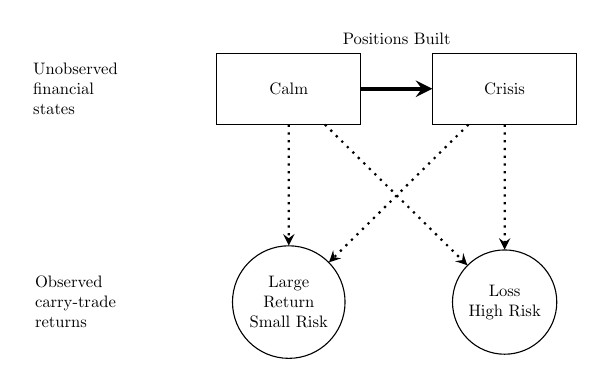
\begin{tikzpicture}[scale = 0.6, transform shape]
\tikzstyle{decision} = [circle, draw, minimum height = 8mm, 
  text width = 5em, text centered];
\tikzstyle{line} = [draw, -stealth, thick]
\tikzstyle{line2} = [draw, -stealth, ultra thick]
\tikzstyle{line3} = [draw, -stealth, dashed, thick]
\tikzstyle{line4} = [draw, -stealth, dotted, thick]
%\tikzstyle{elli} = [draw, ellipse, fill = red!50, minimum height = 8mm, 
 % text width = 5em, text centered]
\tikzstyle{block} = [draw, rectangle, text width = 8em, 
  text centered, minimum height = 15mm, node distance = 8em]
\node [block](Calm){Calm};
%\node [block, left of  = Build, xshift = -5em] (Calm){Calm}; 
\node [block, right  of = Calm, xshift =5em] (Crisis){Crisis};
\node [decision, below of = Calm, yshift = -10em, align = center]
(Calm2) {Large Return \\ Small Risk}; 
\node [decision, below of = Crisis, yshift = -10em](Crisis2) {Loss \\ High Risk};
%\node [decision, below of = Caution, yshift = -10em, align = center](Caution2) 
%{Small \\ Return \\ Average \\ Risk};
%arrows 
%\path [line3] (Calm) -- (Calm);
%\path [line3] (Crisis) -- (Crisis);
%\path [line3] (Crash) -- (Crash2);
\path [line2] (Calm) -- node [yshift = 3em] {Positions Built} (Crisis);
%\path [line2] (Caution) -- node [yshift = 3em]  {Speculative Lending} (Build);
\path [line4] (Calm) -- (Crisis2);
\path [line4] (Crisis) -- (Calm2);
\path [line4] (Calm) -- (Calm2);
\path [line4] (Crisis) -- (Crisis2);
%\path [line4] (Crash) -- (Caution2);
%\path [line4] (Crash) -- (Build2);
\node [align = left, left of = Calm, xshift = -10em] {Unobserved \\ 
financial \\states};
\node [align = left, left of = Calm2, xshift = -10em] {Observed \\ 
carry-trade \\
returns};
%\path [line] (decision1) -| node [yshift = 0.5em, 
%   xshift = 8em] {YES} (process 1);
%\path [line3] (Crash) -- (Caution); 
%   xshift = -8em] {NO} (process 2);
\end{tikzpicture}
\caption{Two-Regime Hidden Markov Model (HMM)}
\label{figref:HMM2}
\end{figure}
\end{frame}

\begin{frame}{Three components of HMM}
The HMM has three components: $\pi, A, B$ where,
\begin{itemize}[<+-| alert@+>]
\pause
\item The prior model: $P(S_1 = n| \theta_{prior})$ $(\pi)$
\item The transition model: $P(S_t| S_{t-1}, \theta_{trans})$ $(A)$
\item The response model: $P(Y_t| S_t, \theta_{resp})$ $(B)$
\end{itemize}
\pause
Where there are $n$ states or regimes; $y_t$ are the observed carry-trade returns; and $\theta_{prior}$, $\theta_{trans}$ and  $\theta_{resp}$ are the parameters of the prior, transition and response models respectively.
\end{frame}

\begin{frame}{Transition matrix}
The transition matrix is
\begin{equation*}
\begin{bmatrix}
P(S_t = 1|S_{t-1}=1),  & P(S_t = 2|S_{t-1}=1)\\
P(S_t = 1|S_{t-1}=2),  & P(S_t = 2|S_{t-1}=2)
\end{bmatrix}
\end{equation*}
For Hungary, it is 
\begin{equation*}
\begin{bmatrix}
0.88,  & 0.12\\
0.42,  & 0.58
\end{bmatrix}
\end{equation*}
\end{frame}

% Note that this frame uses the multirow and the [fixup] argument to push the 
% names of the rows up so that they are not covered by the horizontal lines
\begin{frame}{Response}
For the simple two-regime case, a linear response is modelled as
\begin{equation*}
y_t = \beta_0 + \sum_{i=1}^{i=n}S_{i,t} + \varepsilon_t
\end{equation*}

For, Hungary Poland, Romania and Czech, there are the following results. 
\begin{center}
\rowcolors{1}{OliveGreen!20}{OliveGreen!5}
 \begin{tabular}{lrrrrr}
  \hline
 Regime& & HUF & PLN & CZK & RON \\ 
  \hline
   \multirow{2}{*}[5pt]{Calm}& Mean & 1.0165 & 1.0173 & 1.0129 & 1.0150 \\ 
&St-Dev& 0.0519 & 0.0486 & 0.0542 & 0.0433  \\ 
\hline
\multirow{2}{*}[5pt]{Crash}& Mean & 0.9905 & 0.9862 & 0.9963 & 0.9969  \\ 
 &S-Dev & 0.1085 & 0.1026 & 0.0886 & 0.0878 
\end{tabular}
\end{center}
\end{frame}

\section{Results}
\begin{frame}{The models}
\begin{enumerate}[<+-| alert@+>]
\item Base model $y_t = \beta_1 + \varepsilon_t$ (M1)
\item 2 Regime $y_t = \beta_1 + \sum_{i=1}^{i=n}S_{i,t} + \varepsilon_t, \quad n = 2$ (M2) 
\item 3 Regime $y_t = \beta_1 + \sum_{i=1}^{i=n}S_{i,t} + \varepsilon_t, \quad n = 3$ (M3)
\item 2 Regime Z response $y_t = \beta_1 + \beta_2 Z_t + \varepsilon_t$ (M4)
\item 2 Regime Z transition $y_t = \beta_t + \sum_{i=1}^{i=n}(S_{i,t}|z_t) + \varepsilon_t, \quad n = 2$ (M5) 
\begin{itemize}
\item transition model $log(a_{ij}/ a_{i1}) = \alpha_j +\beta_{j}z_t$
\end{itemize}
\end{enumerate}
\end{frame}

\begin{frame}{Transition and risk aversion}
The VIX is scaled to have a mean of zero and S-dev of 1.  
\begin{center}
\rowcolors{1}{OliveGreen!20}{OliveGreen!5}
\begin{tabular}{rrrrrrr}
  \hline
 & -3sd & -1sd & Mean & +1sd & +2sd & +3sd \\ 
  \hline
  HUF & 0.0020 &  0.0242 & 0.0807 & 0.2375 & 0.5249 & 0.7967 \\ 
  PLN & 0.0004 &  0.0063 & 0.0242 & 0.0887 & 0.2766 & 0.6003 \\ 
  CZK & 0.0000 &  0.0034 & 0.0717 & 0.6367 & 0.9755 & 0.9989 \\ 
  RON & 0.0014 &  0.0131 & 0.0392 & 0.1119 & 0.2799 & 0.5453  
\end{tabular}
\end{center}
The probability of switching to a crash once in a state of calm.
\end{frame}

\begin{frame}{Calm and Crash probabilities}
\includegraphics<1>[width=12cm, height=9cm]{"../../Figures/HUFEUR2"}
\end{frame}

\section{Next steps}
\begin{frame}{Next Steps}
\begin{itemize}[<+-| alert@+>]
\item Repeat this for US monetary policy, international liquidity and availability of credit
\begin{itemize}
\item US short-term interest rate, TED spread, credit
\end{itemize}
\item Common factors and common dates
\item Real time country risk factor
\end{itemize}
\end{frame}

\section{Bibliography}

\begin{frame}[allowframebreaks]{Bibliography}
  \begin{thebibliography}{10}    
  \beamertemplatearticlebibitems
  \bibitem{Calvo}
    G.~Calvo.
    \newblock Capital flows and capital market crisis: the simple economics of sudden stops
    \newblock {\em Journal of Applied Economics}, 1(1):34--54, 1998.
  \bibitem{Ahmed}
    S.~Ahmed and A. Zlate.
    \newblock Capital flows to emerging economies: A brave new world?
    \newblock {\em Journal of International Money and Finance}, 2014.
  \bibitem{Hamilton}
    J.D.~Hamilton.
    \newblock Rational expectations: Econometric analysis of changes in regime
    \newblock {\em Journal of Economic Dynamics and Control}, 12(2):385--423, 1988.
  
  \end{thebibliography}
\end{frame}
\end{document}


